\section{Design of Cerberus}
\label{Sec:Scheduler}

\begin{figure}[htp]
        \centering
        \includegraphics[width=3.6in]{CerberusBBSystem}
        \caption{The design of Three-Phase burst buffer aware scheduling. The black arrows indicate 
        the jobs changing of status; the red, brown and blue arrows in the bottom indicate the data flow in different phases.}
        \label{Fig:CerberusBBSystem}
\end{figure}


\subsection{Three-Phase Job Scheduling}

The traditional batch scheduler on a system without burst buffer only considers
the job with the number of required nodes and the expected runtime
for making the scheduling decisions.
The most commonly used scheduling policy is the First Come First Serve with EASY backfilling~\cite{tsafrir-tpds-2007}.
However, on burst-buffer-enabled systems,
the amount of available burst buffer capacity becomes a new scheduling object.

In this work,
we propose Cerberus, a burst-buffer-aware batch scheduler.
We assume that upon job submission, a user specifies the amount of compute nodes, 
the expected job runtime, and the amount of burst buffer needed by her job.
Cerberus makes scheduling decisions based on the job demands of computing nodes as well as burst buffer.
It allocates burst buffer to each job with regard to its use cases
by maintaining three distinct queues, as shown in Figure~\ref{Fig:CerberusBBSystem}.
The input queue $Q_I$ contains all the jobs that need to prefetch data
from the external storage to the burst buffer.
The running queue $Q_R$ holds the jobs that are waiting for the compute nodes and
the burst buffer used in data exchange for various purposes.
Jobs waiting to be drained out to the external permanent storage are in the output queue $Q_O$.
The layered hierarchy in Figure~\ref{Fig:CerberusBBSystem} also indicates that burst buffer
can fill in the memory gap between the memory on compute nodes and the hard disk storage.
Cerberus coordinates three queues and makes scheduling decisions according to job requirements
in each queue with the objective of maximize job performance and system utilization.

To see how Cerberus schedules a particular job by manipulating three queues,
we present the job transition diagram in Figure~\ref{Fig:JobFSM}.
After the submission, a job enters $Q_I$ waiting for the stage-in-purpose burst buffer ($BB_{in}$).
Once selected by Cerberus, the job is removed from $Q_I$ and start to fetch input data.
After finishing the stage-in phase, the job is enqueued to $Q_R$,
where it waits for the required compute nodes and \textit{new} burst buffer used in running phase($BB_{run}$).
Note that $BB_{in}$ is still held by the job at this time point.
When Cerberus chooses the job from $Q_R$, the job will be put to the running phase.

The first thing to do in running phase is to release $BB_{in}$ after
\textbf{fetching in} data to the memory of the acquired compute nodes.
During the execution, data exchanges between the memory and the burst buffer $BB_{run}$
may occur frequently.
Once the job execution finishes, $BB_{run}$ can be immediately released since
output data are still available on the compute nodes.
Without releasing the compute nodes, the job enters $Q_O$ and waits for a certain amount of burst buffer for staging out its data ($BB_{out}$).

Once a job in $Q_O$ is chosen by Cerberus, its data flow from the main memory to the burst buffer
in the \textbf{drain-out} sub-phase, after which all the compute nodes can be released.
Then the burst buffer nodes are responsible for transferring the output data to the external storage.
The job completes when all its data are staged out and $BB_{out}$ are returned to system.

As indicated by Figure~\ref{Fig:JobFSM}, the resource release at anytime can trigger Cerberus
to schedule jobs in three queues.
The details of how Cerberus makes scheduling decision for each queue are
described in Section~\ref{SubSec:OptStageIn}-\ref{SubSec:OptStageOut}.
%The fine scheduling granularity enables the full utilization of burst buffer for different purposes.
%The divide-conquer approach provides a framework that can be extended to various scheduling
%policies for each individual phase.
%We propose and solve two optimizations targeting $Q_I/Q_O$ and $Q_R$ in Section~\ref{Sec:Opt}

\begin{figure}[htp]
\centering
        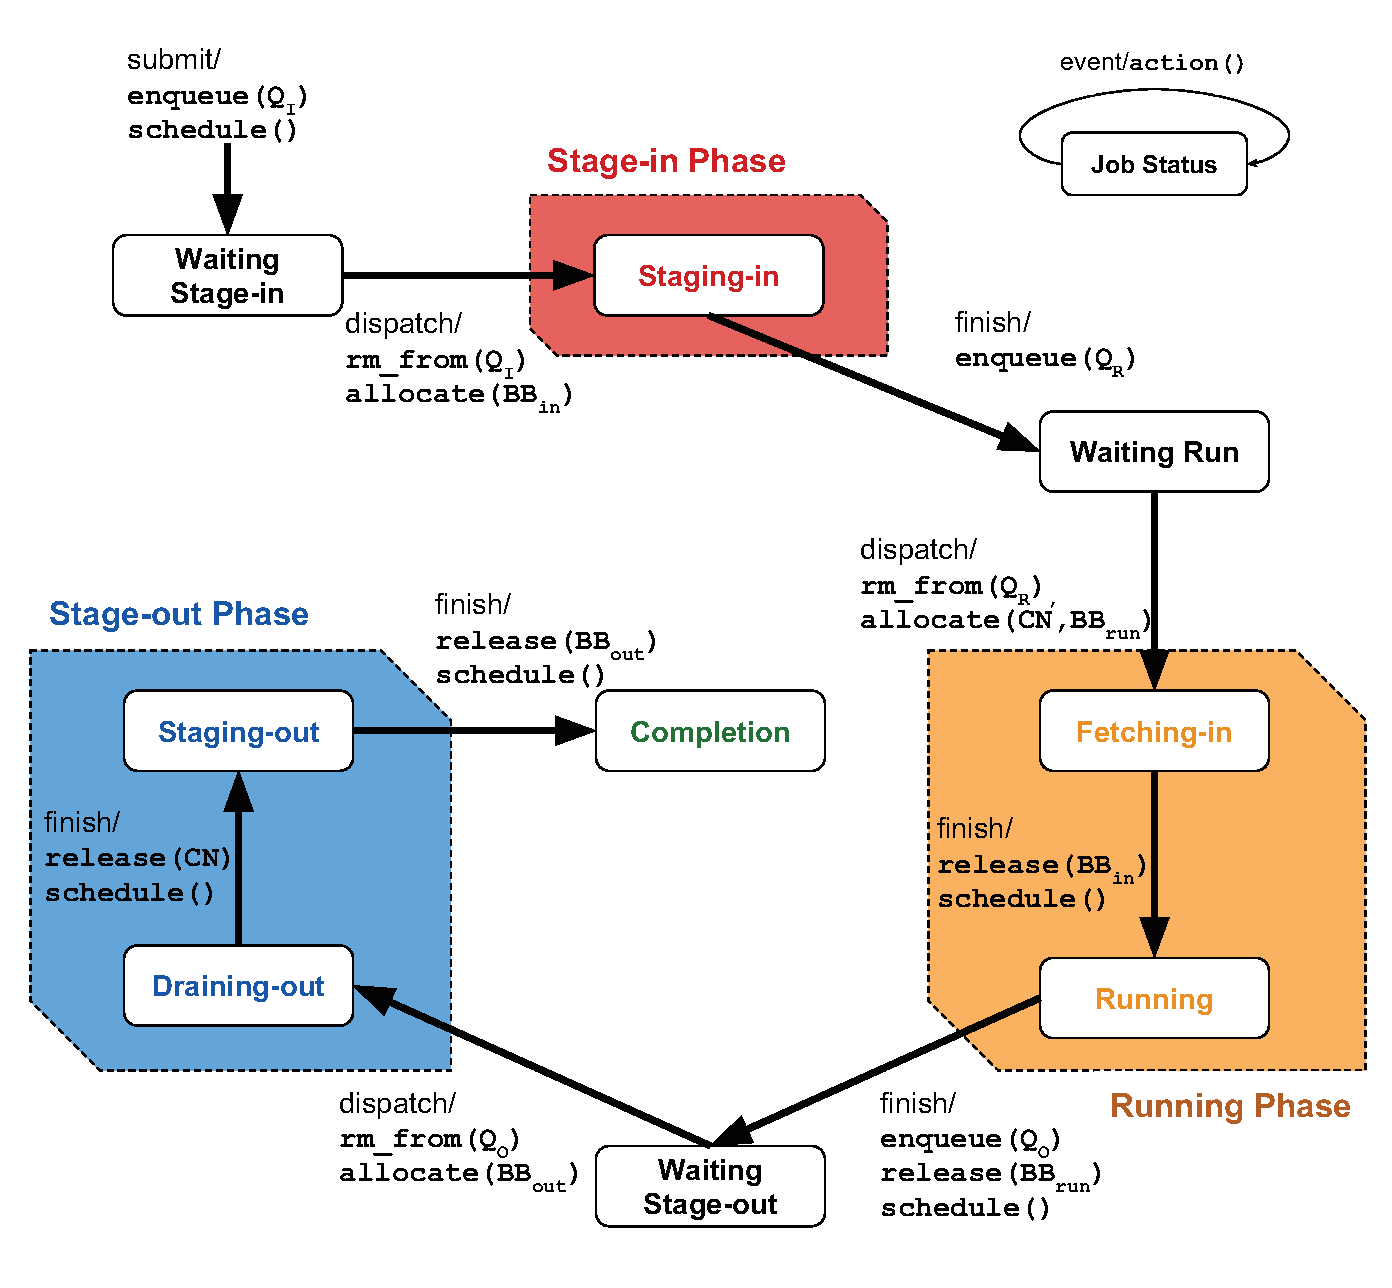
\includegraphics[width=3.6in]{3PhaseJobFSM}
        \caption{Job state transition in Cerberus}
\label{Fig:JobFSM}
\end{figure}

\subsection{Three-Phase Coordination}
\label{SubSec:Coordination}
The three phase model does not assume data independence between the three phases.
Cooperations are necessary in scheduling the three phases.
First, only after finishing the stage-in phase can a job be ready for running.
Similarly, only when finishing the running phase can a job waiting or entering the stage-out phase,
reflected in the lifetime of a job's execution.
This is still true even when input data is so large that it must be read in chunks.
In this case we load the first chunk of data in the stage-in phase so that application
can run with one chunk of data;
meanwhile, the application has to keep reading data in chunks during the running phase.
Notice that for this purpose, we only need burst buffer that is able to hold one chunk
of, instead of whole, input data.
However, this case barely happens because of burst buffer's reasonable capacity\footnote{For
example, 3.7 PB burst buffer on Trinity system should be able to hold most single job's input.}.

Secondly, the burst buffer of any job used at any phase can only be used for a single phase.
For example, a running-phase job cannot hold its already taken burst buffer
and to enter stage-out phase upon finishing the running phase,
regardless whether the holding burst buffer has sufficient capacity.
In Cerberus, the resource release is mandatory as specified in Figure~\ref{Fig:JobFSM}.
We believe that frequent releases provide more opportunities to involve the scheduler in each phase for scheduling the jobs.

Most of the time, data exchanges only occur between main memory and burst buffer in running phase.
This rule breaks when application generates output data more than main memory's capacity.
When this case occurs, we suggest system put output data chunk first from memory to burst buffer
so that application can resume execution with freed memory;
then we let burst buffer node handle the data transfer to external storage.
The stage-out phase handles only the last piece of output data as in normal case.

Finally, it is possible that none of three queues are empty at the moment of a scheduling instance.
We choose a heuristic strategy to determine the scheduling order when
Cerberus has to handle multiple queues at the same time.
Noting that jobs finishing the \textit{running} and the \textit{stage-out} phases will
(partially) release the resources,
we set the priority of queues to be $priority(Q_O) > priority(Q_R) > priority(Q_I)$.
This greedy heuristic works well when the demand of the jobs in $J_{Q_I}$ is low.
However, it is possible to make jobs stack up at the entry of the system,
whose solution is part of our future work.


\subsection{Scheduling in the Stage-in Phase}
\label{SubSec:OptStageIn}

In the stage-in phase, jobs require only the burst buffer.
Cerberus schedules the jobs in $Q_I$ based on their burst buffer demands $bb\_in$.
To maximize burst buffer's utilization, Cerberus schedules the jobs
according to the following optimization:
\begin{align*}
        \mathbf{Problem} & \text{ } \mathbf{1} \\
        \max &\sum_{i\in J_{Q_I}} bb\_in_i \cdot x_i \\
        s.t. &\left\{
                \begin{array}{l}
                        x_i \in \{0, 1\}, \forall i \in J_{Q_I}\\ [0.8em] \numberthis \label{Equ:MaxTransferData}
                        \sum_{i \in J_{Q_I}} bb\_in_i \cdot x_i \leq BB_{available}
                \end{array}
        \right.
\end{align*}
%\begin{align*}
        %& \max \sum_{i\in S} bb\_in_i \\
        %& s.t. \sum_{i\in S} bb\_in_i \leq BB_{available} \numberthis \label{Equ:MaxTransferData}
        %%\left\{
                %%\begin{array}{l}
                        %%S \subseteq J_{Q_I} \\ [1em]
                        %%\sum_{i\in S} bb\_in_i \leq BB_{available}
                %%\end{array} 
        %%\right.
%\end{align*}
where $J_{Q_I}$ contains all the jobs in the input queue,
$bb\_in_i$ is the burst buffer demand of $job_i$,
$BB_{available}$ is the available capacity of the burst buffer at the moment.
We denote the set of jobs that achieve the maximum data transfer throughput as
$\mathcal{J_{Q_I}} = \{i|x_i = 1, \text{ } \forall i \in J_{Q_I}\}$.

Problem 1 is equivalent to the 0-1 knapsack problem, which is NP-complete.
It can be solved in pseudo-polynomial time through dynamic programming and backtracking.
Memorization technique is applied in order to accelerate the solving process.
The recursive relationship used in our solution is given by \equref{Equ:MaxTransferDataRecursion}.
The time complexity of solving \equref{Equ:MaxTransferDataRecursion} and 
backtracking $\mathcal{J}_{Q_I}$ is $O(|Q_I|\times BB_{available})$.


\subsection{Scheduling in the Running Phase}
\label{SubSec:OptRunning}
Running jobs not only require the compute nodes for computation,
but also utilize the burst buffer to enhance the I/O performance.
Here we take a general strategy by defining the \textbf{profit} of $job_i$
in $Q_R$ as it uses $c_i$ compute nodes and $bb\_run_i$ amount of the burst buffer
\begin{equation}
        p_i = f(c_i, bb\_run_i, ert_i)
\label{Equ:GeneralProfit}
\end{equation}
where $ert_i$ is the expected running time of $job_i$.

Cerberus's objective is to maximize the total profit of jobs in the running queue, formularized as
\begin{align*}
        \mathbf{Problem} & \text{ } \mathbf{2} \\
        \max &\sum_{i \in J_{Q_R}} p_i \cdot x_i \\
        s.t. &\left\{
                \begin{array}{l}
                        x_i \in \{0, 1\}, \forall i \in J_{Q_R} \\ [0.8em]
                        \sum_{i \in J_{Q_R}} c_i \cdot x_i \leq CN_{available} \\ [0.8em]\numberthis \label{Equ:MaxProduct} 
                        \sum_{i \in J_{Q_R}} bb\_run_i \cdot x_i \leq BB_{available}
                \end{array} 
        \right.
\end{align*}
where $J_{Q_R}$ contains all the jobs in the running queue,
$CN_{available}$ and $BB_{available}$ represent the amount of system's current available resources.
We denote the set of jobs who have the maximum profit as
$\mathcal{J}_{Q_R}  = \{i|x_i=1, \text{ } \forall i \in J_{Q_R}\}$.

As an example, we measure the value of a job based on how efficient one utilizes its resource:
\begin{equation}
        p_i = \frac{c_i / CN}{ert_i} \times \frac{bb\_run_i / BB}{ert_i}
        \label{Equ:DefValue}
\end{equation}
In \equref{Equ:DefValue}, efficiency is measured as the ratio
of the job resource demand to the expected job running time,
where the share of the requested compute nodes ($c_i/CN$) and
the share of the requested burst buffer ($bb\_run/BB$) are used to
represent the demand size.
Specializing Problem 2 using \equref{Equ:DefValue} in fact favors tasks that claim to take up the resources with a short duration, as we will discuss in Section~\ref{Sec:Experiments}.
%\begin{align*}
        %& \max \sum_{i \in S}\frac{c_i}{ert_i} * \frac{bb\_run_i}{ert_i} \\
        %& s.t. \left\{
                %\begin{array}{l}
                        %%S \subseteq J_{Q_R} \\ [1em]
                        %\sum_{i \in S} c_i \leq CN_{available} \\ [0.5em]\numberthis \label{Equ:MaxProduct} 
                        %\sum_{i \in S} bb\_run_i \leq BB_{available}
                %\end{array} 
        %\right.
%\end{align*}


Problem 2 can be informally treat as the two-dimension 0-1 knapsack problem.
We use the same dynamic programming skill to solve Problem 2.
The recursion is given by \equref{Equ:MaxProductRecursion}.
The time complexity of solving \equref{Equ:MaxProductRecursion} and selecting $\mathcal{J}_{Q_R}$ with memorization technique is $O(|Q_R|\times CN_{available}\times BB_{available})$.


\subsection{Scheduling in the Stage-out Phase}
\label{SubSec:OptStageOut}

The stage-out phase scheduling is designed based on the value of $bb\_out$ of the jobs in $Q_O$.
The optimization formula for the stage-out phase is the same as Problem 1, 
except that $bb\_in_i$ is replaced with $bb\_out_i$, 
and $J_{Q_I}$ is replaced with $J_{Q_O}$, the job set of output queue.
The solution is also extremely similar to \equref{Equ:MaxTransferDataRecursion} and
has the same $O(|Q_O|\times BB_{available})$ time complexity.


%\subsection{Solving the Optimization Problems}
%
%Problem 2 can be informally treat as the 2-dimension 0-1 knapsack problem.
%We expect all of them to be NP-hard problems.
%Dynamic programming is adopted to solve them in pseudo-polynomial time.
%Applying memorization could also help accelerate the solving process.
%In addition, we are not interested in the optimal result of
%Problem 1 and Problem 2,
%but in a combination of jobs $\mathcal{J}$ that yields to the optimal solution,
%which, fortunately, can also be tracked back down using the memorizations stored during the dynamic programming execution.
%
%For Problem 1, the recursive relationship is given by \equref{Equ:MaxTransferDataRecursion}.
%The recursion that solves Problem 2 is given by \equref{Equ:MaxProductRecursion}.
%Solving \equref{Equ:MaxTransferDataRecursion} and 
%backtracking $\mathcal{J}_{Q_I}$ or $\mathcal{J}_{Q_O}$ in total take time proportional to $n\times BB$.
%Similarly, solving \equref{Equ:MaxProductRecursion} and selecting $\mathcal{J}_{Q_R}$ using memo
%are $O(n\times CN\times BB)$.


\begin{strip}
        \begin{align}
                dp(i, w) = & 
                \left\{
                        \begin{array}{l}
                                0, \text{ if $i=0$ } \\ [0.6em]
                                dp(i-1, w), \text{ if $bb\_in_i > w$} \\ [0.6em]
                                \max \{ dp(i-1, w), dp(i-1, w-bb\_in_i) + bb\_in_i \}, \text{ if $bb\_in_i \leq w$}
                        \end{array} 
                \right.
                \label{Equ:MaxTransferDataRecursion} 
        \end{align}
\end{strip}

\begin{strip}
        \begin{align}
                dp(i, c, w) = &
                \left\{
                        \begin{array}{l}
                                0, \text{ if $i=0$ } \\ [0.6em]
                                dp(i-1, c, w), \text{ if $c_i > c$ or $bb\_run_i > w$} \\ [0.6em]
                                \max \{ dp(i-1, c, w), dp(i-1, c - c_i, w - bb\_run_i) + p_i \}, \text{ if $c_i \leq c$ and $bb\_run_i \leq w$}
                        \end{array} 
                \right.
                \label{Equ:MaxProductRecursion}
        \end{align}
\end{strip}

\subsection{Discussion}
The optimal solutions in any of scheduling phases may not be unique;
then backtracking via memoization only yields one of the optimal solution to Problem 1-3.
For example, backtracking $\mathcal{J}_{Q_R}$ using $dp(i,c,w)$ only return 1 scheduling
configuration that maximize our optimization goal.
If the runtime system designer don't specify extra constraints in the scheduling problems,
Cerberus, as any other scheduler, cannot automatically prioritize \textbf{optimal} solutions
because prioritizing using any hidden rules leads to some kind of unfairness.

Another thing to point out is that Cerberus is \textbf{NOT} unfair to non-I/O jobs.
As for Problem 1, a non-I/O job will always be selected by Cerberus.
Since we have $bb_{in} = 0$ for non-I/O jobs, adding it to $\mathcal{J}_{Q_I}$ will affect
neither of the constraints in \equref{Equ:MaxTransferData}.
To avoid starving certain jobs demanding extremely large number of burst buffers and/or cores,
Cerberus keeps tracking of their holding time.
When the waiting time exceed certain threshold, Cerberus will stop the normal scheduling
process to dispatch the large jobs.



